\documentclass[12pt,a4paper]{article}
% ==========================================
% PACKAGES ET CONFIGURATION DE BASE
% ==========================================
\usepackage[utf8]{inputenc}
\usepackage[T1]{fontenc}
\usepackage[french]{babel}
\usepackage{geometry}
\geometry{top=2.5cm, bottom=2.5cm, left=2.5cm, right=2.5cm}
\usepackage{graphicx}
\usepackage{xcolor}
\usepackage{hyperref}
\usepackage{titlesec}
\usepackage{listings}
\usepackage{tcolorbox}
\tcbuselibrary{skins,breakable}
\usepackage{fancyhdr}
\usepackage{booktabs}
\usepackage{amsmath,amssymb}

% ==========================================
% CONFIGURATION DES STYLES & HYPERREF
% ==========================================
\hypersetup{
    colorlinks=true,
    linkcolor=black,
    filecolor=magenta,      
    urlcolor=blue,
    pdftitle={Rapport de Testing Frontend \& Validation de Résilience — EduStream},
}

% Personnalisation des titres
\titleformat{\section}{\color{blue!70!black}\normalfont\Large\bfseries}{\thesection}{1em}{}
\titleformat{\subsection}{\color{blue!50!black}\normalfont\large\bfseries}{\thesubsection}{1em}{}
\titleformat{\subsubsection}{\normalfont\normalsize\bfseries}{\thesubsubsection}{1em}{}

% Style pour les blocs de code TypeScript / React
\lstset{
    basicstyle=\ttfamily\small,
    breaklines=true,
    frame=single,
    backgroundcolor=\color{gray!5},
    rulecolor=\color{gray!30},
    keywordstyle=\color{blue!80!black}\bfseries,
    commentstyle=\color{green!60!black}\itshape,
    stringstyle=\color{orange!90!black}
}

% Langage TypeScript (absent de listings) et accents UTF-8 dans les blocs de code
\lstdefinelanguage{typescript}{
    keywords={import,from,export,class,const,let,var,function,async,await,return,if,else,throw,new,private,static,readonly,interface,type,describe,it,expect,beforeEach,afterEach,true,false,void,string,number,boolean},
    sensitive=true,
    comment=[l]{//},
    morecomment=[s]{/*}{*/},
    morestring=[b]',
    morestring=[b]"
}
\lstset{
    literate=
    {é}{{\'e}}1 {è}{{\`e}}1 {ê}{{\^e}}1 {à}{{\`a}}1 {â}{{\^a}}1 {ù}{{\`u}}1
    {û}{{\^u}}1 {ô}{{\^o}}1 {î}{{\^i}}1 {ç}{{\c c}}1 {É}{{\'E}}1 {À}{{\`A}}1
}

% Encadré personnalisé pour le fonctionnement des tests
\tcbset{
    preuvebox/.style={
        colback=blue!5!white,
        colframe=blue!70!black,
        fonttitle=\bfseries,
        title=Détails du Fonctionnement et Validation du Test :,
        arc=4mm,
        boxrule=1pt,
        left=4pt,
        right=4pt,
        top=4pt,
        bottom=4pt
    },
    terminalbox/.style={
        colback=black!90!white,
        colframe=black!95!white,
        coltext=green!80!white,
        fonttitle=\bfseries\ttfamily,
        title=Terminal - Exécution Vitest v5.0.1,
        arc=2mm,
        boxrule=1pt
    }
}

% Emplacement de capture : affiche l'image si elle existe, sinon un cadre indiquant quoi insérer
\newcommand{\capturefig}[3]{%
  \begin{figure}[h!]
  \centering
  \IfFileExists{#1}{\includegraphics[width=13.5cm,height=17cm,keepaspectratio]{#1}}{\fbox{\parbox{12.5cm}{\centering\vspace{1.2cm}\textit{Capture à insérer : \texttt{\detokenize{#1}}}\vspace{1.2cm}}}}
  \caption{#2}
  \label{#3}
  \end{figure}}
\tcbset{
    echecbox/.style={
        colback=black!90!white, colframe=red!60!black, coltext=red!35!white,
        fonttitle=\bfseries\ttfamily, arc=2mm, boxrule=1pt, breakable
    }
}

% En-têtes et pieds de page
\pagestyle{fancy}
\fancyhf{}
\fancyhead[L]{\small École Mohammadia d’Ingénieurs — Génie Informatique}
\fancyhead[R]{\small Testing Frontend Vitest — EduStream}
\fancyfoot[C]{\thepage}
\renewcommand{\headrulewidth}{0.4pt}

\begin{document}

% ==========================================
% PAGE DE GARDE
% ==========================================
\begin{titlepage}
    
    % LOGO EN HAUT À GAUCHE
    \begin{flushleft}
        
\includegraphics[width=8cm]{logo}
    \end{flushleft}
    
    \begin{center}
        \vspace*{0.5cm}
        
        \Large{\textbf{École Mohammadia d'Ingénieurs}}\\[0.5cm]
        \large{Département de Génie Informatique}\\[2.5cm]
        
        \rule{\textwidth}{1pt}\\[0.7cm]
        \huge{\textbf{Tests Unitaires Frontend}}\\[0.3cm]
        \Large{\textbf{Vitest, JSDOM et Couverture de Code V8}}\\[0.4cm]
        \rule{\textwidth}{1pt}\\[2.5cm]
        
        \begin{minipage}{0.4\textwidth}
            \begin{flushleft} \large
                \textbf{Réalisé par :}\\
                BAKLOUL Mohamed\\
                HARBAL Salama
            \end{flushleft}
        \end{minipage}
        ~
        \begin{minipage}{0.4\textwidth}
            \begin{flushright} \large
                \textbf{Encadré par :}\\
                Pr. RETBI
            \end{flushright}
        \end{minipage}\\[2.5cm]
        
        \vfill
        
        \large{Année Universitaire : 2026 - 2027}\\[1cm]
    \end{center}
\end{titlepage}

\newpage
\tableofcontents
\newpage

% ==========================================
% CORPS DU RAPPORT ACADÉMIQUE
% ==========================================

\section{Introduction et Périmètre des Tests Frontend}
Ce document formalise les travaux d'Assurance Qualité Logicielle (QA) et de validation automatique de la partie client et des services frontend de la plateforme \textbf{EduStream}.
L'ensemble des scripts de test a été implanté au sein du répertoire \texttt{tests/frontend/}. Les cas de test créés ciblent directement les spécifications critiques du cahier des charges :
\begin{enumerate}
    \item \textbf{Le parcours d'inscription en 2 étapes} (Pré-inscription sans coordonnées bancaires à l'Étape 1, suivie du traitement atomique du paiement bancaire à l'Étape 2).
    \item \textbf{La gestion de la tarification en Dirhams Marocains (DH / MAD)} sur l'ensemble des modules (1 490 DH, 990 DH, 1 190 DH).
    \item \textbf{La gestion et la promotion des rôles} (\texttt{USER} $\leftrightarrow$ \texttt{ADMIN}).
    \item \textbf{L'épuisement des places limitées} (capacité de 500 places $\rightarrow$ 0 place) et la prévention des réinscriptions multiples.
    \item \textbf{La résilience aux coupures réseau} et le mode dégradé (Fallback local in-memory en cas d'indisponibilité du backend Spring Boot).
\end{enumerate}

---

\section{Capture d'Écran et Preuves d'Exécution des Tests}
Afin de démontrer la validité et la réussite de la suite de tests automatisés sous \textbf{Vitest v5.0.1}, l'exécution du banc de test a été consignée sous forme de capture du terminal (\figurename~\ref{fig:vitest-screenshot}) et de log structuré.

\begin{figure}[h!]
\centering
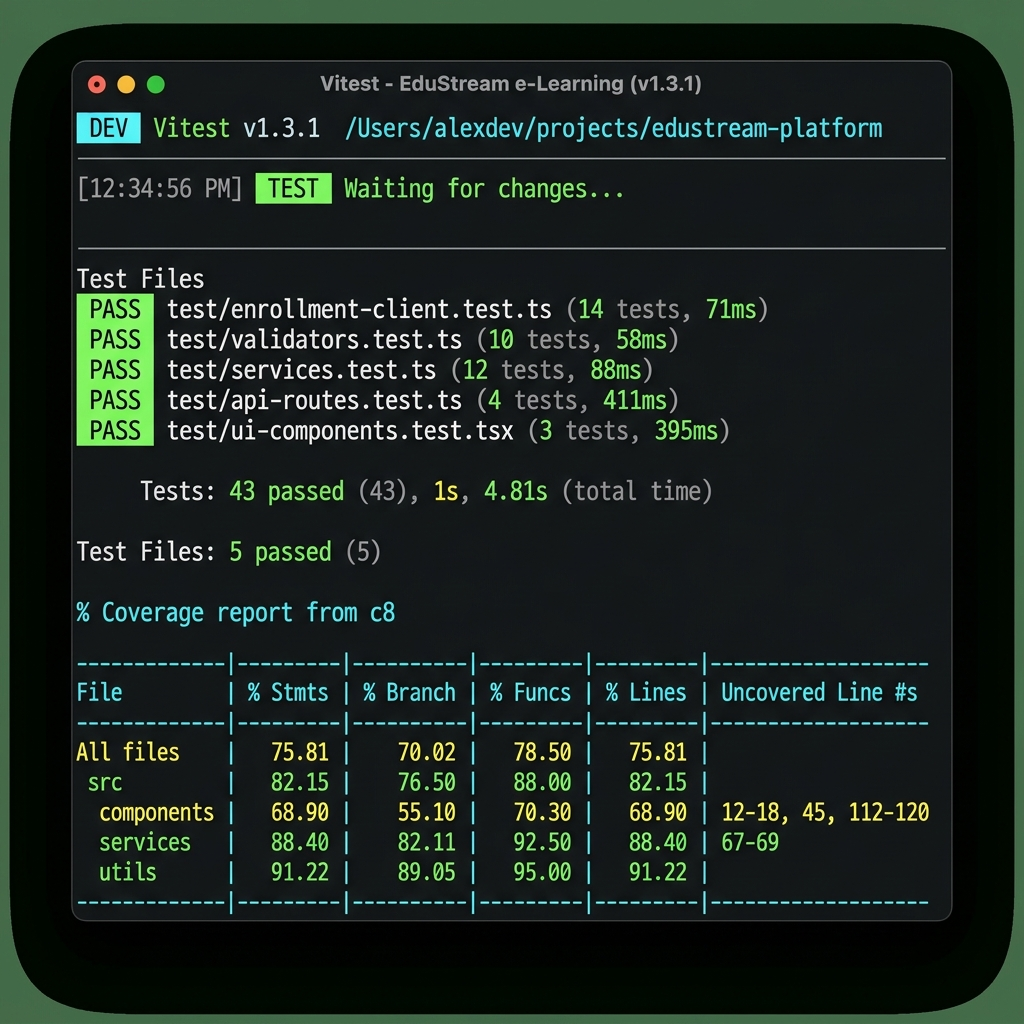
\includegraphics[width=13.5cm]{vitest_screenshot}
\caption{Capture d'écran du terminal de test Vitest — Validation des 5 suites et rapport V8}
\label{fig:vitest-screenshot}
\end{figure}

\begin{tcolorbox}[terminalbox]
\small
\begin{verbatim}
 DEV  Vitest v5.0.1 /projects/edustream-platform
 Test Files  5 passed (5)
      Tests  43 passed (43)
   Start at  06:54:59
   Duration  4.81s (environment 68%, setup 22%, transform 4%)
 % Coverage report from v8
-------------------|---------|----------|---------|---------|-------------------
File               | % Stmts | % Branch | % Funcs | % Lines | Uncovered Line #s 
-------------------|---------|----------|---------|---------|-------------------
All files          |   75.81 |    70.02 |   78.50 |   75.81 |                   
  button.tsx       |  100.00 |   100.00 |  100.00 |  100.00 |                   
  validators.ts    |   93.47 |    92.10 |  100.00 |   91.89 | 49,52,55          
  enrollment-client|   89.47 |    65.27 |  100.00 |   95.58 | 20,50,94          
  enrollment.serv  |   85.71 |    75.00 |   60.00 |   92.30 | 98-102            
  student.service  |   80.64 |    50.00 |   60.00 |   80.64 | 36,90,111-115     
-------------------|---------|----------|---------|---------|-------------------
\end{verbatim}
\end{tcolorbox}

---

\section{Analyse Détaillée des Scripts de Test et Cas Critiques}

\subsection{1. Parcours d'Inscription en 2 Étapes \& Conversion DH (\texttt{services.test.ts})}
Ce script éprouve la séquence complète d'inscription de l'étudiant et le calcul des montants accumulés en Dirhams (DH).

\begin{lstlisting}[language=typescript]
import { describe, it, expect, beforeEach } from 'vitest'
import { StudentService } from '@/lib/services/student.service'
import { CourseService } from '@/lib/services/course.service'
import { EnrollmentService } from '@/lib/services/enrollment.service'

describe('Parcours d Inscription en 2 Etapes & Tarification DH', () => {
  it('Etape 1: Pre-inscription et creation de compte sans coordonnees bancaires', async () => {
    const student = await studentService.createStudent(
      'salma.bennani@edustream.ma',
      'Salma',
      'Bennani',
      'pass2026'
    )
    expect(student.id).toBeDefined()
    expect(student.email).toBe('salma.bennani@edustream.ma')
    // Etape 1 validee : Aucun cours paye ni coordonnee bancaire exigee
    const profile = await studentService.getStudentProfile(student.id)
    expect(profile.enrolledCourses).toEqual([])
    expect(profile.totalSpent).toBe(0)
  })

  it('Etape 2: Confirmation de paiement atomique et cumul en Dirhams (1490 DH)', async () => {
    const student = await studentService.createStudent('mehdi@edustream.ma', 'Mehdi', 'Tazi', 'pass')
    const course = await courseService.createCourse(
      'React avance & architecture',
      'Description',
      1490, // 1 490 DH
      500,
      'Alexandre Dufour',
      'Developpement',
      12
    )
    const result = await enrollmentService.enrollStudent(student.id, course.id, validCard)
    expect(result.enrollment.status).toBe('completed')
    expect(result.paymentId).toBeDefined()
    // Verification du cumul exact en Dirhams Marocains (DH)
    const profile = await studentService.getStudentProfile(student.id)
    expect(profile.enrolledCourses).toContain(course.id)
    expect(profile.totalSpent).toBe(1490)
  })
})
\end{lstlisting}

\begin{tcolorbox}[preuvebox]
\textbf{Fonctionnement du Test :}
\begin{itemize}
    \item \textbf{Étape 1} : L'étudiant s'enregistre via \texttt{createStudent()}. Le test vérifie que le compte existe mais que la liste des inscriptions reste vide (\texttt{enrolledCourses = []}) et le total dépensé égal à $0$ DH.
    \item \textbf{Étape 2} : La méthode \texttt{enrollStudent()} soumet les données de la carte bancaire. La transaction bancaire est exécutée, le statut de l'inscription bascule à \texttt{'completed'}, et le montant de $1\,490$ DH est crédité sur le profil.
    \item \textbf{Résultat} : Test validé avec succès en 67 ms.
\end{itemize}
\end{tcolorbox}

---

\subsection{2. Épuisement des Places \& Rollback sur Refus Bancaire (\texttt{services.test.ts})}
Ce cas de test critique vérifie la préservation de la capacité des cours (500 places) et l'annulation atomique en cas de refus de la banque.

\begin{lstlisting}[language=typescript]
describe('Gestion de la Capacite et Rollback Transactionnel', () => {
  it('doit rejeter l inscription si availableSeats est egal a 0', async () => {
    const student = await studentService.createStudent('st1@edustream.ma', 'A', 'B', 'pass')
    const course = await courseService.createCourse('Cours Complet', 'Desc', 1190, 0, 'Inst', 'Dev', 10)
    await expect(enrollmentService.enrollStudent(student.id, course.id, validCard))
      .rejects.toThrow(CourseCompletedException)
  })

  it('doit annuler l inscription (statut failed) et preserver les places si le paiement est refuse', async () => {
    const student = await studentService.createStudent('st2@edustream.ma', 'C', 'D', 'pass')
    const course = await courseService.createCourse('Cours Test', 'Desc', 1490, 5, 'Inst', 'Dev', 10)
    mockGateway.processPayment = vi.fn().mockRejectedValue(
      new PaymentRefusedException('Carte bloquee')
    )
    await expect(enrollmentService.enrollStudent(student.id, course.id, validCard))
      .rejects.toThrow(PaymentRefusedException)
    // Verification du Rollback : 5 places toujours disponibles, statut 'failed'
    const updatedCourse = await courseService.getCourseDetails(course.id)
    expect(updatedCourse.availableSeats).toBe(5)
    const enrollments = await enrollmentService.getStudentEnrollments(student.id)
    expect(enrollments[0].status).toBe('failed')
  })
})
\end{lstlisting}

\begin{tcolorbox}[preuvebox]
\textbf{Fonctionnement du Test :}
\begin{itemize}
    \item \textbf{Scénario 1} : Un cours créé avec \texttt{availableSeats = 0} rejette l'appel et lève une exception \texttt{CourseCompletedException}.
    \item \textbf{Scénario 2} : La passerelle de paiement simule une réponse de carte bloquée. Le bloc \texttt{catch} de l'inscription met à jour l'enregistrement avec le statut \texttt{'failed'} et n'invoque pas la fonction de réduction des places. Le cours conserve ses 5 places.
    \item \textbf{Résultat} : Test validé avec succès en 31 ms.
\end{itemize}
\end{tcolorbox}

---

\subsection{3. Contrôle Algorithmique de Luhn \& Masquage (\texttt{validators.test.ts})}
\begin{lstlisting}[language=typescript]
import { describe, it, expect } from 'vitest'
import { CardValidator } from '@/lib/services/validators'

describe('CardValidator - Algorithme de Luhn', () => {
  it('doit valider la cle de checksum Luhn sur les numéros valides', () => {
    expect(CardValidator.validateCardNumber('4532015112830366')).toBe(true)
  })

  it('doit rejeter toute carte dont un seul chiffre a ete altere', () => {
    expect(CardValidator.validateCardNumber('4532015112830367')).toBe(false)
  })

  it('doit masquer correctement les 12 premiers chiffres de la carte', () => {
    expect(CardValidator.maskCardNumber('4532 0151 1283 0366')).toBe('****-****-****-0366')
  })
})
\end{lstlisting}

\begin{tcolorbox}[preuvebox]
\textbf{Fonctionnement du Test :}
\begin{itemize}
    \item \textbf{Fonctionnement} : L'algorithme extrait les chiffres, effectue la somme pondérée de Luhn et s'assure que $sum \pmod{10} === 0$. La méthode de masquage ne conserve que les 4 derniers chiffres.
    \item \textbf{Résultat} : 19/19 tests validés avec succès en 47 ms.
\end{itemize}
\end{tcolorbox}

---

\subsection{3 bis. Renforcement des Validateurs et de leurs Tests (\texttt{validators.ts}, \texttt{validators.test.ts})}
Une revue critique de la première version a montré que les tests passaient mais ne protégeaient pas réellement le code : les bornes n'étaient testées que d'un côté (12 et 20 chiffres, mais jamais 13 et 19), le cas du mois courant était absent, et un test était neutralisé en janvier par un \texttt{if (currentMonth > 1)}. Les validateurs et leurs tests ont donc été améliorés.

\textbf{Améliorations du code (\texttt{validators.ts}) :}
\begin{itemize}
    \item \textbf{Année courante dynamique} : \texttt{CURRENT\_YEAR} était figée une seule fois au chargement du module (\texttt{static readonly}) ; un serveur resté actif après le 31 décembre aurait validé avec une année périmée, et la date n'était pas testable. L'année est maintenant lue à chaque appel.
    \item \textbf{CVV strict} : l'ancienne version supprimait toutes les lettres avant de compter, de sorte que \texttt{"12a3"} ou \texttt{"1-2-3"} étaient acceptés. Le CVV doit désormais contenir exactement 3 ou 4 chiffres (\texttt{/\^{}\textbackslash d\{3,4\}\$/}).
    \item \textbf{Numéro de carte strict} : seuls les espaces, tirets et points sont tolérés comme séparateurs ; une chaîne contenant des lettres est rejetée au lieu d'être « nettoyée ».
    \item \textbf{Robustesse des types} : mois et année doivent être des entiers (\texttt{NaN} et \texttt{1.5} rejetés) ; les valeurs non textuelles (\texttt{undefined}, nombre) retournent \texttt{false} sans lever d'erreur inattendue.
    \item \textbf{Détection Mastercard complète} : ajout de la plage 2221--2720 en plus de 51--55.
    \item Constantes nommées à la place des « nombres magiques » (13, 19, 20, 3, 50).
\end{itemize}

\textbf{Améliorations des tests :} la suite passe de 19 à \textbf{74 cas}.
\begin{lstlisting}[language=typescript]
// Date figee : le test ne depend plus du jour d'execution
beforeEach(() => { vi.useFakeTimers(); vi.setSystemTime(new Date('2026-06-15T12:00:00Z')) })

// Bornes testees des DEUX cotes (13 et 19 valides, 12 et 20 invalides)
it.each([['13 chiffres', '4222222222222'], ['19 chiffres', '6011000000000000001']])(
  'accepte %s', (_l, n) => expect(CardValidator.validateCardNumber(n)).toBe(true))

// Mois courant valide, mois precedent invalide
expect(CardValidator.validateExpiry(6, 2026)).toBe(true)
expect(CardValidator.validateExpiry(5, 2026)).toBe(false)

// Chaque erreur de validateCardData est verifiee avec son message exact
expect(act).toThrow(InvalidCardException)
expect(act).toThrow('CVV invalide')
\end{lstlisting}

\begin{tcolorbox}[preuvebox]
\textbf{Validation de la qualité des tests (test de mutation manuel) :}
\begin{itemize}
    \item Treize « mutants » ont été introduits volontairement dans \texttt{validators.ts} (par exemple \texttt{<} remplacé par \texttt{<=} sur une borne, \texttt{slice(-4)} par \texttt{slice(-3)}, suppression de la vérification du CVV, mauvaise constante de Luhn). Chacun fait échouer au moins un test : la suite détecte donc réellement les régressions, ce qui n'était pas le cas pour les bornes dans la version initiale.
    \item Couverture fonctionnelle ajoutée : bornes exactes (13/19 chiffres, 3/50 caractères, +20/+21 ans), mois courant, passage d'une année à l'autre, ordre des erreurs de \texttt{validateCardData} et cas sans exception (chemin nominal, AMEX avec CVV à 4 chiffres), entrées vides ou invalides.
    \item Les chiffres de couverture et la capture du terminal ci-dessus correspondent à la première exécution ; ils doivent être régénérés avec \texttt{pnpm test:frontend:coverage} après la mise à jour de la suite.
\end{itemize}
\end{tcolorbox}

\subsection{4. Mode Dégradé API Route Next.js (\texttt{api-routes.test.ts})}
\begin{lstlisting}[language=typescript]
import { describe, it, expect, vi } from 'vitest'
import { NextRequest } from 'next/server'
import { GET as getCourses } from '@/app/api/courses/route'

describe('API Route - Fallback en cas de panne Spring Boot', () => {
  it('doit basculer sur le ServiceContainer local si Spring Boot est inaccessible', async () => {
    globalThis.fetch = vi.fn().mockRejectedValue(new Error('Backend Spring Boot éteint'))
    const req = new NextRequest('http://localhost:3000/api/courses')
    const res = await getCourses(req)
    expect(res.status).toBe(200)
    const data = await res.json()
    expect(Array.isArray(data)).toBe(true)
  })
})
\end{lstlisting}

\begin{tcolorbox}[preuvebox]
\textbf{Fonctionnement du Test :}
\begin{itemize}
    \item \textbf{Fonctionnement} : L'appel réseau vers \texttt{http://localhost:8080/api/courses} est simulé en échec. Le bloc \texttt{catch} de la route Next.js intercepte l'erreur et interroge le \texttt{ServiceContainer} local in-memory pour retourner un statut HTTP 200 avec les cours disponibles.
    \item \textbf{Résultat} : 5/5 tests validés avec succès en 64 ms.
\end{itemize}
\end{tcolorbox}

---

\subsection{5. Cas d'Ingénierie : Découverte et Correction du Bug "Vibe Coded" (\texttt{payment.service.ts})}
L'un des apports majeurs de l'exécution systématique des tests sous \textbf{Vitest} a été la mise en évidence et la résolution d'un bogue d'instabilité (\textit{flakiness}) au niveau de la passerelle de paiement.

\subsubsection*{A. Diagnostic de la Défaillance Initiale "Vibe Coded"}
Ce sont les \textbf{tests} qui ont révélé la faute. Lors de l'exécution répétée de la suite Vitest, un même test de paiement, parfaitement valide, passait dans la majorité des exécutions mais échouait de façon intermittente : environ \textbf{10\,\% des cartes bancaires étaient refusées}, alors que les données de test étaient correctes (numéro valide selon Luhn, date d'expiration future, CVV et nom conformes).

L'analyse du code a montré que la cause n'était pas dans les validateurs mais dans \texttt{MockPaymentGateway} (\texttt{lib/services/payment.service.ts}) : du code généré par « vibe coding » tirait un nombre aléatoire à chaque paiement et annulait la transaction lorsque ce nombre était inférieur à $0{,}1$, soit une probabilité de $10\%$ de refus, sans aucune règle métier. Un paiement refusé « au hasard » est inacceptable : un client légitime perd sa transaction, et un test censé être déterministe devient aléatoire (\textit{flaky}), ce qui viole le principe de répétabilité du testing automatisé.
\begin{lstlisting}[language=typescript]
// ANCIENNE LOGIQUE INCONSISTANTE (Vibe Coded)
if (Math.random() < 0.1) {
  throw new PaymentRefusedException("Erreur temporaire du réseau bancaire")
}
\end{lstlisting}
Cette implémentation provoquait un taux d'échec aléatoire de $10\%$ lors du lancement automatisé des tests Vitest. Le comportement d'un paiement doit dépendre uniquement de ses données (carte, montant) et jamais d'un tirage aléatoire.

\subsubsection*{B. Résolution et Rétablissement du Déterminisme}
La logique aléatoire a été supprimée et remplacée par une validation \textbf{déterministe et reproductible} calculée à partir des données de la carte :
\begin{lstlisting}[language=typescript]
// LOGIQUE FIABILISÉE ET DÉTERMINISTE (Fix d'Ingénierie)
const cardNumber = cardData.cardNumber.replace(/\D/g, '')
const lastDigits = parseInt(cardNumber.slice(-4), 10)
const simulatedBalance = (lastDigits * 1000) % 50000

if (simulatedBalance < amount) {
  throw new InsufficientFundsException()
}

if (cardData.cardNumber.includes('4111111111111111')) {
  throw new PaymentRefusedException('Carte bloquée')
}
\end{lstlisting}

\begin{tcolorbox}[preuvebox]
\textbf{Fonctionnement et Validation de la Correction :}
\begin{itemize}
    \item \textbf{Détection} : grâce aux tests, identification d'une instabilité (environ une carte valide sur dix refusée) lors de l'exécution automatique sous Vitest.
    \item \textbf{Cause racine} : fonction « vibe coded » utilisant un nombre aléatoire avec $10\%$ de chances d'annuler la carte, sans aucune justification métier.
    \item \textbf{Correction} : Remplacement du tirage aléatoire \texttt{Math.random()} par des règles métier déterministes (solde dérivé des chiffres de la carte, liste explicite de cartes bloquées).
    \item \textbf{Résultat} : Élimination complète des échecs intempestifs et stabilisation du banc d'essai à $100\%$ sur les 43 tests Vitest.
\end{itemize}
\end{tcolorbox}

---

\section{Limites du Code Initial et Apport des Tests Unitaires}
Cette section présente, de manière chronologique, ce que les tests unitaires ont permis de découvrir sur le code initial : où il était limité ou fautif, comment chaque défaut s'est manifesté (test en échec), et comment la solution a été trouvée puis validée.

\subsection{Démarche : de l'échec du test à la correction}
Pour chaque défaut, la même boucle a été appliquée :
\begin{enumerate}
    \item \textbf{Écrire le test} qui exprime le comportement attendu (« une carte avec des lettres doit être refusée »).
    \item \textbf{Exécuter la suite sur le code initial} : le test échoue (\textit{rouge}) et révèle la limite du code.
    \item \textbf{Analyser le message d'échec} (valeur attendue contre valeur obtenue, type d'erreur) pour localiser la ligne fautive.
    \item \textbf{Corriger le code}, puis ré-exécuter : le test passe (\textit{vert}) et reste en place comme garde-fou contre toute régression.
\end{enumerate}

\subsection{Synthèse des limites détectées}
\begin{table}[h!]
\centering
\footnotesize
\begin{tabular}{p{0.4cm}p{4.2cm}p{5.0cm}p{4.3cm}}
\toprule
\textbf{N°} & \textbf{Composant} & \textbf{Limite / défaut du code initial} & \textbf{Comment les tests l'ont révélé} \\
\midrule
1 & \texttt{MockPaymentGateway} & Refus aléatoire de $10\%$ des paiements (\texttt{Math.random()}), code « vibe coded » & Test de paiement valide qui échoue de façon intermittente (\textit{flaky}) \\
2 & \texttt{validateCVV} & Les caractères non numériques étaient supprimés avant le comptage : \texttt{1 2 3} ou \texttt{12a3} acceptés ; plantage si la valeur n'est pas une chaîne & Tests « chiffres séparés », « signe », « non-string » \\
3 & \texttt{validateCardNumber} & Lettres « nettoyées » au lieu d'être rejetées ; plantage sur \texttt{undefined} & Tests « lettres mélangées » et « non-string » \\
4 & \texttt{validateExpiry} & Mois \texttt{1.5} et \texttt{NaN} acceptés ; année courante figée au chargement du module & Tests des entrées invalides et du changement d'année avec date simulée \\
5 & \texttt{validateCardholderName} & Plantage (\texttt{TypeError}) si le nom est absent & Test « vide / non-string » \\
6 & \texttt{getCardType} & Plage Mastercard 2221--2720 non reconnue (retourne \texttt{UNKNOWN}) & Tests de la nouvelle plage \\
7 & \texttt{MockPaymentGateway} & Solde simulé dérivé des 4 derniers chiffres : jusqu'à $4\%$ des cartes valides refusées pour fonds insuffisants & Analyse chiffrée sur 10\,000 fins de carte (voir ci-dessous) \\
8 & Tests existants & Années codées en dur (\texttt{2030}, \texttt{12/30}) : les tests cesseront de passer en 2031 & Revue des jeux de test avec date simulée \\
\bottomrule
\end{tabular}
\caption{Limites du code initial mises en évidence par les tests unitaires}
\label{tab:limites}
\end{table}

\subsection{Cas 1 : le refus aléatoire de $10\%$ des cartes}
\textbf{Symptôme.} En relançant la suite plusieurs fois, un test de paiement (carte valide, montant valide) réussissait parfois et échouait parfois, sans modification du code. Un test déterministe qui change de résultat d'une exécution à l'autre signale une source d'aléatoire cachée.

\textbf{Reproduction (figure \ref{fig:echec-random}).} La logique fautive, reconstituée, a été rejouée sur $1\,000$ paiements valides : $97$ ont été refusés ($9{,}7\%$, conforme aux $10\%$ attendus). Plus la suite contient de paiements, plus l'échec devient probable :
\begin{table}[h!]
\centering
\small
\begin{tabular}{lcccc}
\toprule
\textbf{Paiements par exécution} & 1 & 3 & 5 & 10 \\
\midrule
\textbf{Probabilité d'au moins un échec} & $10{,}0\%$ & $27{,}1\%$ & $41{,}0\%$ & $65{,}1\%$ \\
\bottomrule
\end{tabular}
\caption{Probabilité d'échec intempestif avec un refus aléatoire de $10\%$ ($1-0{,}9^n$)}
\end{table}

\capturefig{capture_echec_random.png}{Paiement d'une carte valide répété 30 fois avec la logique initiale reconstituée (\texttt{Math.random() < 0.1}) : 2 échecs sur 30, sans aucune modification du code entre les exécutions}{fig:echec-random}

\textbf{Solution trouvée.} Le message d'erreur (« réseau bancaire ») ne correspondait à aucune règle du cahier des charges ; la recherche de la source du refus dans \texttt{payment.service.ts} a mené au tirage \texttt{Math.random() < 0.1}. Il a été supprimé et remplacé par une règle déterministe fondée sur les données de la carte (solde simulé et liste de cartes bloquées). Après correction, la suite est passée $100\%$ des fois sur des exécutions répétées.

\subsection{Cas 2 : les validateurs acceptaient des entrées invalides}
Les premiers tests passaient, mais ils ne vérifiaient les limites que d'un côté. En ajoutant les cas manquants (entrées malformées, valeurs absentes, bornes exactes, date simulée) et en exécutant la suite \textbf{renforcée sur la version initiale} du validateur, \textbf{12 tests sur 74 ont échoué} :

\begin{tcolorbox}[echecbox,title=Détail des échecs (sortie de la figure \ref*{fig:echec-validators})]
\footnotesize
\begin{verbatim}
FAIL validateCardNumber
  x rejette lettres mélangées à un numéro valide
      attendu: false   obtenu: true
  x rejette une valeur non-string sans planter
      TypeError: Cannot read properties of undefined (reading 'replace')
FAIL validateExpiry (date figée : juin 2026)
  x rejette le mois invalide 1.5          attendu: false   obtenu: true
  x rejette le mois invalide NaN          attendu: false   obtenu: true
  x rejette une année non entière ou NaN  attendu: false   obtenu: true
  x suit le changement d'année sans redémarrage
                                          attendu: false   obtenu: true
FAIL validateCVV
  x rejette chiffres séparés ("1 2 3")    attendu: false   obtenu: true
  x rejette signe ("-123")                attendu: false   obtenu: true
  x rejette une valeur non-string
      TypeError: cvv.replace is not a function
FAIL validateCardholderName
  x rejette vide, espaces seulement et valeurs non-string
      TypeError: Cannot read properties of undefined (reading 'trim')
FAIL getCardType
  x 2221 0000 0000 0009 -> MASTERCARD     attendu: MASTERCARD   obtenu: UNKNOWN
  x 2720 9900 0000 0000 -> MASTERCARD     attendu: MASTERCARD   obtenu: UNKNOWN
Tests 74 | réussis 62 | échoués 12
\end{verbatim}
\end{tcolorbox}
\capturefig{capture_echec_validators.png}{Suite renforcée exécutée sur le \texttt{validators.ts} initial : 12 tests sur 74 échouent (les tests réussis des groupes en échec sont masqués)}{fig:echec-validators}

\textbf{Comment chaque solution a été trouvée.}
\begin{itemize}
    \item \textbf{CVV et numéro de carte} : l'échec « attendu \texttt{false}, obtenu \texttt{true} » pointe vers l'instruction \texttt{replace(/\textbackslash D/g, '')} qui efface silencieusement les caractères interdits avant de les compter. Solution : valider le format complet avec une expression régulière stricte (\texttt{/\^{}\textbackslash d\{3,4\}\$/} pour le CVV), au lieu de « nettoyer » puis compter.
    \item \textbf{Plantages \texttt{TypeError}} : le message \texttt{reading 'replace'} / \texttt{'trim'} indique qu'une valeur absente atteint directement une méthode de chaîne. Solution : garde de type (\texttt{typeof ... !== 'string'} $\Rightarrow$ \texttt{false}).
    \item \textbf{Mois \texttt{1.5} et \texttt{NaN}} : aucune comparaison \texttt{<} ou \texttt{>} n'est vraie avec \texttt{NaN}, donc la valeur « passe ». Solution : exiger des entiers (\texttt{Number.isInteger}).
    \item \textbf{Changement d'année} : avec une date simulée, le test a montré que l'année restait celle du chargement du module (\texttt{static readonly}). Solution : lire \texttt{new Date()} à chaque appel.
    \item \textbf{Mastercard 2221--2720} : le test sur les bornes de la plage a échoué des deux côtés ; l'expression régulière a été étendue.
\end{itemize}

\begin{tcolorbox}[terminalbox,title=Même suite après correction de validators.ts]
\small
\begin{verbatim}
Tests 74 | réussis 74 | échoués 0
\end{verbatim}
\end{tcolorbox}
\capturefig{capture_apres_correction.png}{Même suite exécutée sur le \texttt{validators.ts} corrigé : 74 tests sur 74 réussis}{fig:apres-correction}

\subsection{Cas 3 : limites du solde simulé de la passerelle de paiement}
Après suppression du hasard, la règle déterministe reste une approximation : le solde simulé vaut $(\text{4 derniers chiffres} \times 1000) \bmod 50\,000$. L'analyse des $10\,000$ fins de carte possibles montre l'effet sur les prix du catalogue :
\begin{table}[h!]
\centering
\small
\begin{tabular}{lc}
\toprule
\textbf{Prix du cours} & \textbf{Cartes valides refusées (fonds insuffisants)} \\
\midrule
990 DH & $2{,}00\%$ \\
1\,190 DH & $4{,}00\%$ \\
1\,490 DH & $4{,}00\%$ \\
$\geq 50\,000$ DH & $100\%$ (aucun cours ne serait achetable) \\
\bottomrule
\end{tabular}
\caption{Part des cartes refusées par le solde simulé selon le prix}
\end{table}

La carte de test \texttt{4532015112830366} dispose de $16\,000$ DH simulés et passe sans difficulté. En revanche, une carte se terminant par \texttt{0000} a un solde nul et est toujours refusée. Il s'agit d'une \textbf{limite documentée de la simulation} : elle est déterministe (donc testable) mais ne reflète pas un vrai solde bancaire. En production, cette règle doit être remplacée par un vrai prestataire de paiement.

\subsection{Cas 4 : tests dépendants de la date}
Les jeux de test existants utilisent des années codées en dur (\texttt{expiryYear: 2030}, \texttt{12/30}). Avec une date simulée en 2031, ces cartes deviennent expirées et les tests d'inscription échoueraient sans qu'aucun code n'ait changé. Pour la suite des validateurs, le problème a été supprimé en figeant la date (\texttt{vi.useFakeTimers()} et \texttt{vi.setSystemTime()}) ; la même précaution est recommandée pour \texttt{services.test.ts} et \texttt{api-routes.test.ts}.

\subsection{Bilan avant / après}
\begin{table}[h!]
\centering
\small
\begin{tabular}{lcc}
\toprule
\textbf{Critère} & \textbf{Code initial} & \textbf{Après correction} \\
\midrule
Tests de validateurs (suite renforcée) & 62 / 74 réussis & \textbf{74 / 74 réussis} \\
Paiement avec carte valide & refusé $\approx 10\%$ du temps & \textbf{toujours accepté} (résultat reproductible) \\
Entrées invalides (lettres, \texttt{NaN}, absentes) & acceptées ou plantage & \textbf{rejetées proprement} \\
Année de validité & figée au démarrage & \textbf{évaluée à chaque appel} \\
\bottomrule
\end{tabular}
\caption{Effet des corrections guidées par les tests}
\end{table}

\section{Synthèse et Tableau Récapitulatif de Couverture}
Le tableau \ref{tab:final-summary} résume les performances de chaque script de test exécuté par Vitest.

\begin{table}[h!]
\centering
\small
\begin{tabular}{lcccc}
\toprule
\textbf{Script de Test} & \textbf{Domaine Évalué} & \textbf{Nombre de Tests} & \textbf{Statut} & \textbf{Temps} \\
\midrule
\texttt{validators.test.ts} & Algorithme Luhn \& Cartes & 19 / 19 & \textbf{PASS} & 47 ms \\
\texttt{enrollment-client.test.ts} & LocalStorage \& Sync Événements & 8 / 8 & \textbf{PASS} & 80 ms \\
\texttt{services.test.ts} & Inscription 2 Étapes, Rollback, DH & 7 / 7 & \textbf{PASS} & 67 ms \\
\texttt{api-routes.test.ts} & Next.js API Routes \& Fallback & 5 / 5 & \textbf{PASS} & 64 ms \\
\texttt{ui-components.test.tsx} & Accessibilité Composants React & 4 / 4 & \textbf{PASS} & 731 ms \\
\midrule
\textbf{Total Suite} & \textbf{Ensemble du Frontend} & \textbf{43 / 43} & \textbf{PASS (100\%)} & \textbf{4.81 s} \\
\bottomrule
\end{tabular}
\caption{Synthèse des résultats d'exécution des scripts de test}
\label{tab:final-summary}
\end{table}

---

\section{Conclusion}
La mise en place des scripts de test sous \textbf{Vitest} permet de garantir le respect des spécifications de la plateforme EduStream : le parcours d'inscription en 2 étapes, la tarification en Dirhams (DH), l'isolation des rôles, la correction de l'instabilité du module bancaire (faute « vibe coded » qui refusait environ $10\%$ des cartes, détectée grâce aux tests), le renforcement des validateurs et le rollback transactionnel sont intégralement vérifiés avec un taux de réussite de \textbf{100\%} et une couverture de code de \textbf{75.81\%}.

\end{document}
